\begin{lead}

 前章において$z$変換を用いたシステムの伝達関数の表現について説明した.この伝達関数によって,システムの安定性や周波数特性を知ることができる.本章ではその方法について説明する.

\end{lead}

\chapter[システムの安定性と周波数特性]{システムの安定性と\\周波数特性}

\label{chapter:42}

\section{逆$z$変換とシステムの安定性}

ここでは,\ref{section:3-2}節の説明とは逆に,$z$変換$X(z)$から\index{りさんじかんしんごう@離散時間信号}離散時間信号$x(n)$を求める方法について説明し,システムの\index{あんていせい@安定性}安定性にも言及する.

\subsection{逆$z$変換}

いま,$X(z)$の\index{ぎゃくzへんかん@逆$z$変換}逆$z$変換を次式のように表す.
\begin{equation}
x(n)=Z^{-1}[X(z)]
\end{equation}
この逆$z$変換は,次式に示すような複素積分により求められる.
\begin{equation}
x(n)=\frac{1}{2\pi j} \oint_C X(z)z^{n-1}dz
\end{equation}
ここで,\index{せきぶんろ@積分路}積分路$C$は,収束領域内で原点を内部に含む反時計方向の円周路である.

この式で計算することが厳密ではあるが,実際には以下に示すような方法によって簡単に逆$z$変換が可能である.

\subsubsection{べき級数展開法}

ここでは,$z$の\index{べききゅうすう@べき級数}べき級数に展開し逆$z$変換を行う方法である,\index{べききゅうすうてんかいほう@べき級数展開法}べき級数展開法について説明する.

次式に示すような$z$変換から明らかではあるが,$X(z)$が$z$の多項式(べき級数)で与えられる場合,離散時間信号$x(n)$は各$z$の係数に対応する.
\begin{equation}
X(z)=\sum_{n=-\infty}^{\infty}x(n)z^{-n}
\label{eqn:eqn-3-1b}
\end{equation}

たとえば,
\begin{equation}
X(z)=\frac{1}{3}(1+z^{-1}+z^{-2})
\label{eqn:eqn-3-1c}
\end{equation}
のような3点平均の場合の逆$z$変換は,
\begin{equation}
x(n)=Z^{-1}[X(z)]=\frac{1}{3}(\delta(n)+\delta(n-1)+\delta(n-2))
\label{eqn:eqn-3-1c1}
\end{equation}
と容易に求められる.

もうひとつの例として,
\begin{equation}
X(z)=\frac{1}{1-bz^{-1}}
\label{eqn:eqn-3-1d}
\end{equation}
の逆変換を求める.この場合は,初項1,公比$bz{-1}$の等比級数を意味することから,

\begin{eqnarray}
X(z) = \frac{1}{1-bz^{-1}} %\nonumber \\
 = 1+bz{-1}+b^2z{-2}+b^3z{-3}+ \cdots %\nonumber \\
 = \sum_{n=0}^{\infty}b^nz{-n} \label{eqn:eqn-3-35}
\end{eqnarray}\vskip.3\baselineskip

\noindent とおくことができるので,求める逆$z$変換は\footnote{単位ステップ関数$u(n)$は,
$\displaystyle u(n)=\sum_{k=0}^{\infty}\delta(n-k) \nonumber$である.},

\begin{eqnarray}
x(n)&=&Z^{-1}(X(z)) \nonumber \\
 &=& Z^{-1}[ 1+bz^{-1}+b^2z^{-2}+b^3z^{-3}+ \cdots ] %\nonumber \\
 =  \delta(n)+b\delta(n-1)+b^2\delta(n-2) + \cdots  \nonumber \\
 &=& \sum_{k=0}^{\infty}b^k\delta(n-k) %\\
 = b^n\sum_{k=0}^{\infty}\delta(n-k) %\\
 = b^nu(n)
\end{eqnarray}\vskip.3\baselineskip

\noindent となる.ただし,$u(n)$は\index{たんいすてっぷかんすう@単位ステップ関数}単位ステップ関数である.

また,このように\index{とうひきゅうすう@等比級数}等比級数であるかどうか不明な場合などは,以下に示すような除算を行うことでも求められる.
\[
\begin{array}{lllllll}
 & & 1+ & bz^{-1}+ & bz^{-2}+ & b^{3}z^{-3}+ & \cdots \\ \cline{2-6}
1-bz^{-1} & \bigg) &  1  &  &  &  \\
 & & 1-& bz^{-1} & & & \\ \cline{3-4}
 & &  & bz^{-1} & & & \\
 & &  & bz^{-1}- & b^2z^{-2} & & \\ \cline{4-5}
 & &  &  & b^2z^{-2} & & \\ 
 & &  &  & b^2z^{-2} &-b^{3}z^{-3} & \\ \cline{5-6}
 & &  &  &  &-b^{3}z^{-3} & \\ 
\end{array}
\]

いずれの場合であっても,式(\ref{eqn:eqn-3-35})の逆$z$変換は,次式のように表される.
\begin{equation}
x(n)=Z^{-1}[X(z)]=b^nu(n)
\label{eqn:eqn-3-37}
\end{equation}


\subsubsection{\index{ぶぶんぶんすうてんかいほう@部分分数展開法}部分分数展開法}

より一般的な形の関数であるところの逆$z$変換を考える.いま,次式の逆$z$変換を行うことを例として説明する.
\begin{equation}
X(z)=\frac{1}{1-3z^{-1}+2z^{-2}}
\end{equation}

この式は,分母が因数分解できるので,以下のように部分分数展開をすることができる.

\begin{eqnarray}
X(z)&=&\frac{1}{1-1.5z^{-1}+0.5z^{-2}} \nonumber \\
 &=&\frac{1}{(1-0.5z^{-1})(1-z^{-2})} \nonumber \\
 &=&\frac{1}{(1-0.5z^{-1})}+\frac{2}{(1-z^{-2})} 
\end{eqnarray}\vskip.3\baselineskip

この式を逆$z$変換すると,式(\ref{eqn:eqn-3-37})を用いれば,

\begin{eqnarray}
z(n)&=&Z^{-1}[X(z)] \nonumber \\
 &=&Z^{-1} \left [ \displaystyle \frac{1}{(1-0.5z^{-1})}+\frac{2}{(1-z^{-2})} \right ] \nonumber \\
 &=&-(0.5)^{n}u(n)+2u(n)
\end{eqnarray}\vskip.3\baselineskip

\noindent と求められる.

このように,高次の関数を部分分数展開すると,複数個の低次な逆変換の問題に帰着することができる.

\subsection{安定判別と周波数特性}

伝達関数の\index{あんていはんべつ@安定判別}安定判別を行う方法について述べる.線形シフト不変システムの安定判別は,\index{いんぱるすおうとう@インパルス応答}インパルス応答を用いて行える.インパルス応答の絶対値和が有限であるとき,すなわち,
\begin{equation}
\sum_{n=-\infty}^{\infty}|h(n)|<\infty
\end{equation}
が成立するとき,システムは安定する.

ただ,この式を用いる方法は無限個のインパルス応答を用いて安定判別を行うため,簡単なものではない.
%
ここでは,伝達関数の極を用いることで,無限個のインパルス応答ということを意識せずに安定判別を行える方法を示す.

\subsubsection{システムの安定判別}

伝達関数はインパルス応答を$z$変換したものであるから,逆に,伝達関数を逆$z$変換すればインパルス応答を求めることができる.

たとえば,
\begin{equation}
H(z)=\frac{1}{1-bz^{-1}}
\end{equation}
の逆$z$変換となるインパルス応答は,
\begin{equation}
h(n)=b^n u(n)
\end{equation}
である.このシステムが安定であるためには,
\begin{equation}
|b|<1
\end{equation}
であればよい.この$b$の値は伝達関数の極でもあるので,逆$z$変換を行う前に,極の大きさから同じ結論を導くことは容易である.

また,
\begin{equation}
H(z)=\frac{A_1}{1-b_1z^{-1}}+\frac{A_2}{1-b_2z^{-1}}
\end{equation}
なる伝達関数を考える.ここで,$A_1$, $A_2$は定数である.これは2次の伝達関数を部分分数展開したものであり,$b_1$, $b_2$は極である.

このインパルス応答は逆$z$変換によって求められ,
\begin{equation}
h(n)=A_1(b_1)^n u(n)+A_2(b_2)^n u(n)
\end{equation}
となる.この場合,システムが安定であるためには,
\begin{equation}
|b_1|<1, |b_2|<1
\end{equation}
であればよいことから,2つの極の大きさがともに1より小さければよい.

以上のように,伝達関数の逆$z$変換を行う前に極の大きさを求めることによって,安定なシステムであるかどうかを知ることができる.結論として.伝達関数すべての極の絶対値が1より小さいときにそのシステムは安定となる.これを図\ref{fig:zu-3-9}に示すと,複素平面上ですべての極が単位円の内側に位置することが,システムが安定であるということとなる.

\begin{figure}[H]
\begin{center}
\begin{minipage}{.4\textwidth}
\begin{center}
%\includegraphics[width=9cm]{fig/zu-3-9.eps}
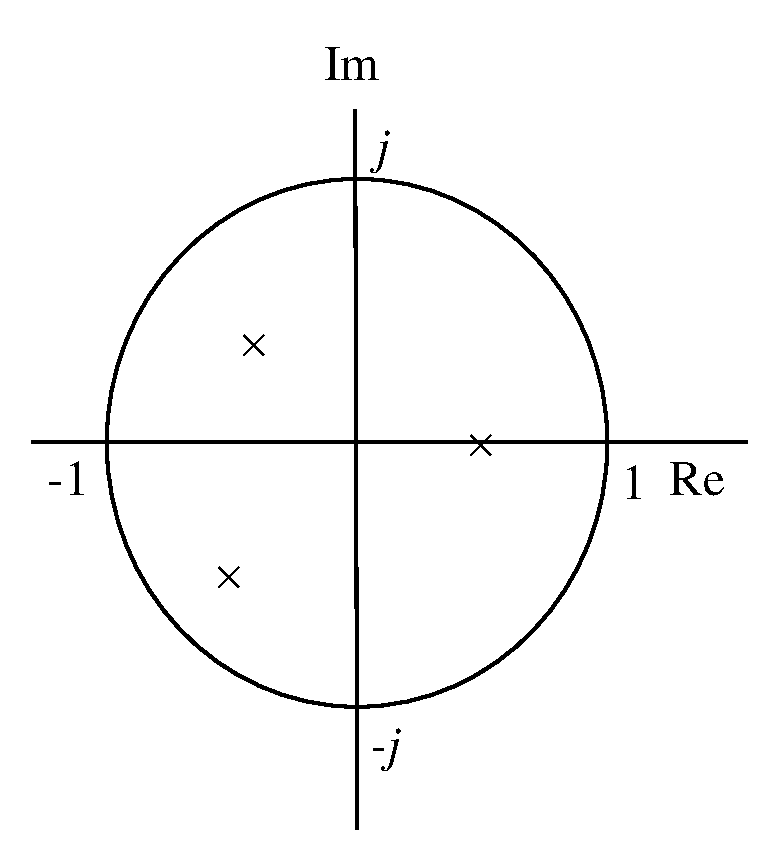
\includegraphics[width=.95\textwidth]{fig/zu-3-9-a.eps}

(a) 安定の例\\(×がすべて単位円の内にある)
\end{center}
\end{minipage}
\begin{minipage}{.4\textwidth}
\begin{center}
%\includegraphics[width=9cm]{fig/zu-3-9.eps}
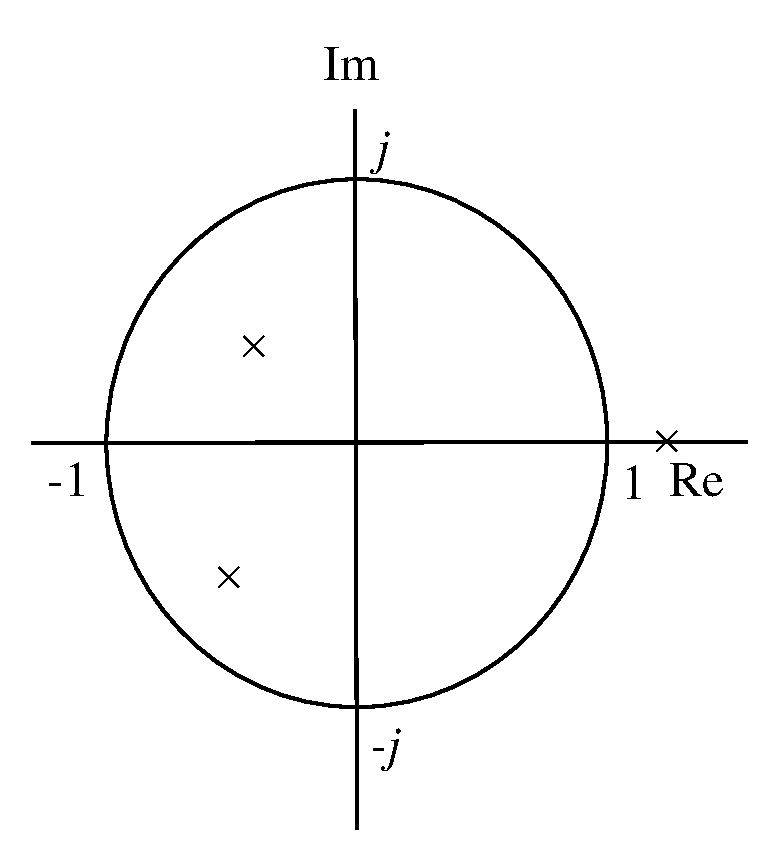
\includegraphics[width=.95\textwidth]{fig/zu-3-9-b.eps}

(b) 不安定の例\\(×が1つでも単位円の外にある)
\end{center}
\end{minipage}
\end{center}\vskip.5\baselineskip
\caption{安定なシステムの\index{きょくはいち@極配置}極配置($\times$は極)}
\label{fig:zu-3-9}
\end{figure}

\section{システムの周波数特性}

ここでは,システムの周波数特性として,\index{しんぷくとくせい@振幅特性}振幅特性と\index{いそうとくせい@位相特性}位相特性,\index{ふくそせいげんはしんごう@複素正弦波信号}複素正弦波信号入力,伝達関数と周波数特性との関係について説明する.

\subsection{振幅特性と周波数特性}

図\ref{fig:zu-3-10}に示す線形時不変システムでは,正弦波信号$x(n)=\cos (\omega n)$を入力したとき,出力信号は$y(n)=A(\omega ) \cos (\omega n + \theta (\omega))$と与えられる.すなわち,以下のような特徴がある.
\begin{enumerate}
\item 出力も同じ周波数$\omega$を持つ正弦波信号である.
\item システムは正弦波信号の大きさ$A(\omega)$と位相$\theta(\omega)$だけを変化させる働きがある.
\item 大きさ$A(\omega)$と位相$\theta(\omega)$はm周波数$\omega$の関数であり,入力信号の周波数により値が異なる.
\end{enumerate}

\begin{figure}[H]
\begin{center}

\includegraphics[width=9cm]{fig/zu-3-10.eps}
\end{center}
\caption{線形時不変システムの入出力関係}
\label{fig:zu-3-10}
\end{figure}

ここで,入力と出力の大きさ(振幅)の関係$A(\omega)$を振幅特性(amplitude characteristics),位相の関係$\theta(\omega)$を位相特性(phase characteristics)という.また,システムの周波数特性 (frequency characteristics)とは,振幅特性と位相特性との両方を含む表現である.

このように,もし,すべての周波数についてシステムの周波数特性を調べることができれば,任意の正弦波信号に対する出力をその結果から容易に知ることが可能となる.また,正弦波信号以外の入力に対する出力も,この周波数特性から決定される.つまり周波数特性は,インパルス応答や伝達関数と同様に,線形時不変システムのすべての能力を表現している.

\subsection{複素正弦波信号入力}

複素正弦波信号として
\begin{equation}
x(n)=e^{j\omega n}= \cos (\omega n) +j\sin (\omega n)
\end{equation}
に対する出力を考える.たたみ込みの式にこの$x(n)$を代入し,整理すると,

\begin{eqnarray}
y(n)&=&\sum_{k=-\infty}^{\infty}h(k)x(n-k) \nonumber \\
 &=&\sum_{k=-\infty}^{\infty}h(k)e^{j\omega (n-k)} \nonumber \\
 &=&e^{j\omega n} \sum_{k=-\infty}^{\infty}h(k)e^{-j\omega k} 
\end{eqnarray}\vskip.3\baselineskip

\noindent ここで,

\begin{eqnarray}
H(e^{j\omega})&=&\sum_{k=-\infty}^{\infty}h(k)e^{-j\omega k} \label{eqn:eqn-3-49}\\
 &=&A(\omega)e^{j\theta(\omega)} \label{eqn:eqn-3-50}
\end{eqnarray}\vskip.3\baselineskip

\noindent とおくと,$y(n)$は,

\begin{eqnarray}
y(n)&=&e^{j\omega n} \sum_{k=-\infty}^{\infty}h(k)e^{-j\omega k} \\
&=&e^{j\omega n} A(\omega)e^{j\theta(\omega)} \\
&=&A(\omega)e^{j(\omega n+\theta(\omega))} \\
&=&A(\omega) \cos (\omega n+\theta(\omega)) +jA(\omega) \sin (\omega n+\theta(\omega))
\end{eqnarray}\vskip.3\baselineskip

\noindent を得ることができる.
この式は,以下に示すことを意味する.
\begin{enumerate}
\item システムの線形性から,複素正弦波に対する出力信号も,\index{せいげんはしんごう@正弦波信号}正弦波信号同様に大きさと信号のみが入力信号と異なる.
\item 式(\ref{eqn:eqn-3-49})を計算し,式(\ref{eqn:eqn-3-50})の式の変形を行えば,大きさと位相の特性を入力信号と独立に知ることができる.
\end{enumerate}

このことから,任意の正弦波信号に対する入出力関係を,式(\ref{eqn:eqn-3-49})に基づいてインパルス応答を用いて計算できることがわかる.

ここで,式(\ref{eqn:eqn-3-49})における$H(\omega)$を周波数特性,それを式(\ref{eqn:eqn-3-50})のように\index{きょくざひょうけいしき@極座標形式}極座標形式に表現したときの大きさ$A(\omega)$を振幅特性,偏角$\theta(\omega)$を位相特性と呼ぶ.


\section{伝達関数と周波数特性}

ここでは,具体的な周波数特性の計算法を説明する.その計算法は,インパルス応答を用いた計算と,伝達関数を用いた計算に大別される.

\subsection{インパルス応答を用いた計算}

インパルス応答$h(n)$が既知である場合に,

\begin{eqnarray}
H(e^{j\omega})&=&\sum_{k=-\infty}^{\infty}h(k)e^{-j\omega k} 
\end{eqnarray}\vskip.3\baselineskip

\noindent のように$n$に代わって$e^{j\omega}$を代入して計算することで,周波数特性を求めることができる.FIRシステムではこの方法でも求めることが可能であるが,IIRシステムの場合は無限個のインパルス応答を扱う必要があるため,決して容易な方法とはいえない.

\subsection{伝達関数を用いた計算}

伝達関数$H(z)$が既知である場合,その$z$に$e^{j\omega}$を代入して計算する.すなわち,
\begin{equation}
H(e^{j\omega})=H(z)|_{z=e^{j\omega}}
\end{equation}
により,周波数特性を求めることができる.

この理由を証明する.まず,インパルス応答の$z$変換が伝達関数となるので,
\begin{equation}
X(z)=\sum_{n=-\infty}^{\infty}x(n)z^{-n}
\label{eqn:eqn-3-1-1}
\end{equation}
の$x(n)$に$h(n)$,$z$に$e^{j\omega}$をそれぞれ代入することによって,

\begin{eqnarray}
H(e^{j\omega})&=&\sum_{k=-\infty}^{\infty}h(k)e^{-j\omega k} 
\end{eqnarray}\vskip.3\baselineskip

\noindent となり,これは式(\ref{eqn:eqn-3-49})と一致する.すなわち,伝達関数の$z$に$e^{j\omega}$を代入した結果と,式(\ref{eqn:eqn-3-49})を直接計算した結果がそれぞれ一致する.また,$e^{j\omega}$の値は複素平面上の単位円周上の値に対応する.

\subsection{周波数特性の描き方}

周波数特性,すなわち振幅特性と位相特性を描く方法については自由度があり,いくつかの方法がある.
%
ここでは,\index{3てんへいきん@3点平均}3点平均のシステム
\begin{equation}
y(n)=\frac{1}{3}(x(n)+x(n-1)+x(n-2))
\end{equation}
を例として説明する.

このシステムの周波数特性は,

\begin{eqnarray}
H(e^{j\omega})&=&\frac{1}{3}(1+e^{-j\omega}e^{-2j\omega}) \nonumber \\
 &=&\frac{1}{3}(e^{j\omega}+1+e^{-j\omega})e^{-j\omega} \nonumber \\
 &=&\frac{1}{3}(e^{j\omega}+e^{-j\omega}+1)e^{-j\omega} \nonumber \\
 &=&\frac{1}{3}(2\cos \omega +1)e^{-j\omega}
\end{eqnarray}\vskip.3\baselineskip

\noindent であるから,振幅特性$A(\omega)$,位相特性$\theta(\omega)$は,
\begin{equation}
A(\omega)=\frac{1}{3}(2\cos \omega +1), \theta(\omega)=-\omega
\label{eqn:eqn-3-56}
\end{equation}
となることから,これを図示すると図\ref{fig:zu-3_15}における点線のようになる.ここで,$\theta(\omega)=-\omega$は原点を通る傾き$-1$の直線であるが,三角関数の周期性$e^{-j\omega}=e^{-j(\omega+2\pi)}$が成立するので,$-\pi \leq \theta(\omega) \leq \pi$の範囲で位相特性を描いている.


\begin{figure}[b]
\begin{center}
\begin{minipage}{.4\textwidth}
\begin{center}
%\includegraphics[width=10cm]{fig/zu-3-15.eps}
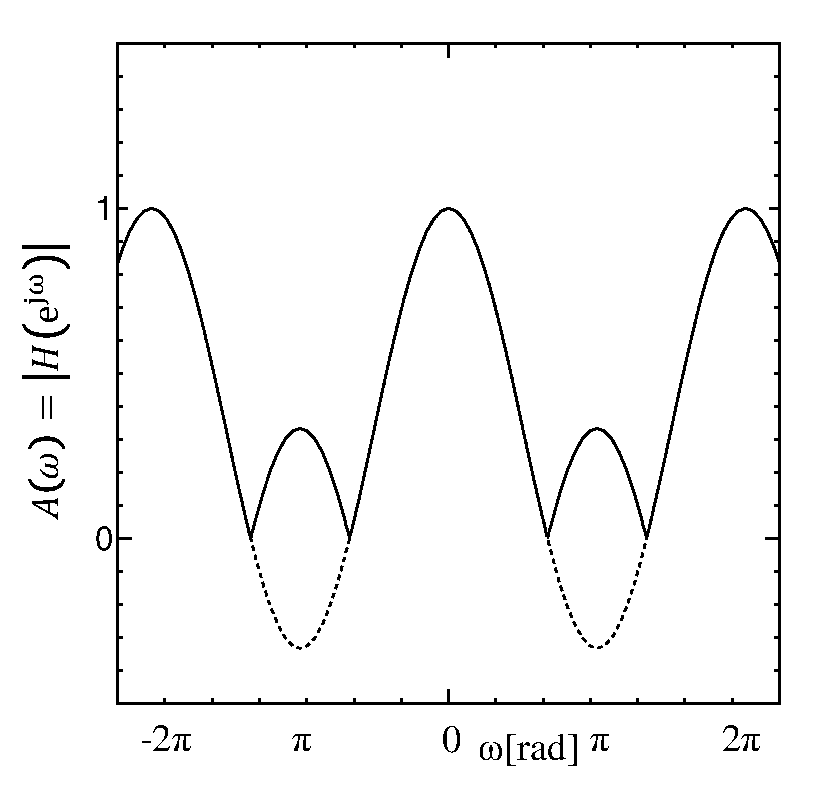
\includegraphics[width=.95\textwidth]{fig/zu-3-15-a.eps}

(a) 振幅特性
\end{center}
\end{minipage}
\begin{minipage}{.4\textwidth}
\begin{center}
%\includegraphics[width=10cm]{fig/zu-3-15.eps}
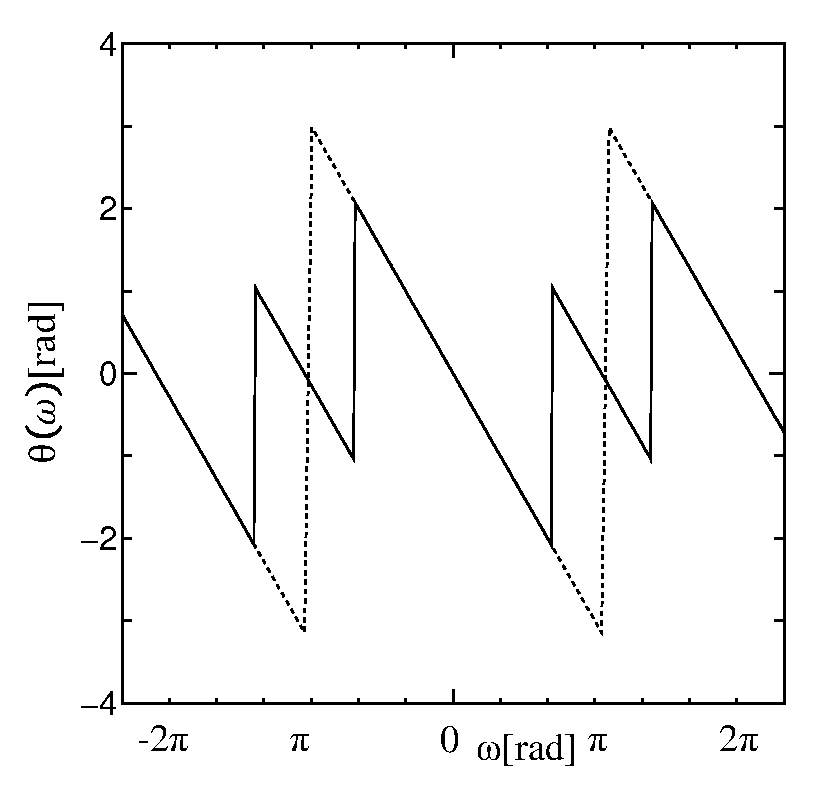
\includegraphics[width=.95\textwidth]{fig/zu-3-15-b.eps}

(b) 位相特性
\end{center}
\end{minipage}
\end{center}\vskip.5\baselineskip
\caption{周波数特性の描き方}
\label{fig:zu-3_15}
\end{figure}

振幅特性について見ると,式(\ref{eqn:eqn-3-56})における$A(\omega)$は実数であるが,$\omega$の値によって正にも負にもなる.しかしながら,振幅特性として$A(\omega)=|H(e^{j\omega})|$を用いる場合には,図\ref{fig:zu-3_15}における実線のように周波数特性を描くことができる.この場合は,$e^{j\pi}=-1$の関係から$A(\omega)$が負になる周波数範囲では位相が$\pi$[rad]変化するので,位相特性も変化する.


\subsection{周波数特性}\index{しゅうはすうとくせい@周波数特性}

図\ref{fig:zu-3_15}に示すように,振幅特性と位相特性ともに,$\omega=2\pi$で周期的な特性をとることがわかる.これは,線形時不変システムにおいては常に成立する性質である.

この性質は,
\begin{equation}
e^{j\omega}=e^{j(\omega+2\pi)}
\end{equation}
が成立することから,
\begin{equation}
H(e^{j\omega})=H(e^{j(\omega+2\pi)})
\end{equation}
が成り立つことによって説明される.

ここで,$\omega=\Omega/F_s=2\pi F/F_s$であることから,周期$\omega=2\pi$は非正規化表現において\index{さんぷりんぐしゅうはすう@サンプリング周波数}サンプリング周波数$F=F_s$に対応する.


また,負の周波数範囲($\omega<0$)についても説明する.一般的に正弦波信号$x(t)=\cos \Omega t$の周波数$\Omega$は1秒間の周期数に相当することから,負の周波数は現実的にあり得ない.ところが,\index{おいらーのこうしき@オイラーの公式}オイラーの公式によるとこの正弦波信号は,
\begin{equation}
\cos \Omega t = \frac{e^{j\Omega t}+e^{-j\Omega t}}{2}
\end{equation}
と書くことができるから,正弦波信号の周波数が正の値をもっていても,対応する複素正弦波信号は負の周波数($-\Omega$)を持つ.このように,周波数特性が複素正弦波信号に基づくことを考えれば,周波数特性図においては負の周波数には意味があることがわかる.

さらに,図\ref{fig:zu-3_15}からわかるように,振幅特性は$\omega=0$で偶対称,位相特性は$\omega=0$で奇対称であるといえる.すなわち,\index{いんぱるすおうとう@インパルス応答}インパルス応答が実数値をとるとき,以下のような関係が常に成立する.
\begin{equation}
A(\omega)=A(-\omega)
\label{eqn:eqn-3-59}
\end{equation}
\begin{equation}
\theta(\omega)=-\theta(\omega)
\label{eqn:eqn-3-60}
\end{equation}

したがって,周期性と式(\ref{eqn:eqn-3-59})ならびに式(\ref{eqn:eqn-3-60})より,インパルス応答が実数のシステムの周波数特性は,$0 \leq \omega < \pi$の範囲でのみ独立であることがわかる.この結論から,ディジタルシステムが処理の対象とする入力信号の周波数は,サンプリング周波数の半分までである.このことは,シャノンのサンプリング定理と同じことと帰着する.

\section{システムの縦続型構成と並列型構成}

\subsection{縦続型構成}

図\ref{fig:zu-3-17}(a)のように2つのシステムを構成することを,\index{じゅうぞくがたこうせい@縦続型構成}縦続型構成という.たとえば,
\begin{equation}
H_1(z)=H_2(z)=\frac{1}{3}(1+z^{-1}+z^{-2})
\label{eqn:eqn-3-61}
\end{equation}
である場合には,3点平均を計算した結果に対して再度3点平均を計算することを意味する.この処理全体をひとつの伝達関数$H(z)$として示すならば,

\begin{eqnarray}
H(z)&=&H_1(z)H_2(z)
\end{eqnarray}\vskip.3\baselineskip

\noindent と書くことができて,図\ref{fig:zu-3-17}(b)のように示すことができる.ここで,$H_1(z)$ならびに$H_2(z)$が式(\ref{eqn:eqn-3-61})の場合には,

\begin{eqnarray}
H(z)&=&H_1(z)H_2(z) \nonumber \\
 &=&\frac{1}{9}(1+z^{-1}+z^{-2})(1+z^{-1}+z^{-2}) \nonumber \\
 &=&\frac{1}{9}(1+2(z^{-1}+z^{-2})+(z^{-1}+z^{-2})^2) \nonumber \\
 &=&\frac{1}{9}(1+2z^{-1}+2z^{-2}+z^{-2}+2z^{-3}+z^{-4}) \nonumber \\
 &=&\frac{1}{9}(1+2z^{-1}+3z^{-2}+2z^{-3}+z^{-4})
\end{eqnarray}\vskip.3\baselineskip

\noindent となる.このような場合,$H_1(z)$と$H_2(z)$が逆の順番であったとしても,$H_1(z)H_2(z)$に変化はないことがわかる.この性質はたたみ込みの交換則から説明される.

\begin{figure}[H]
\begin{center}
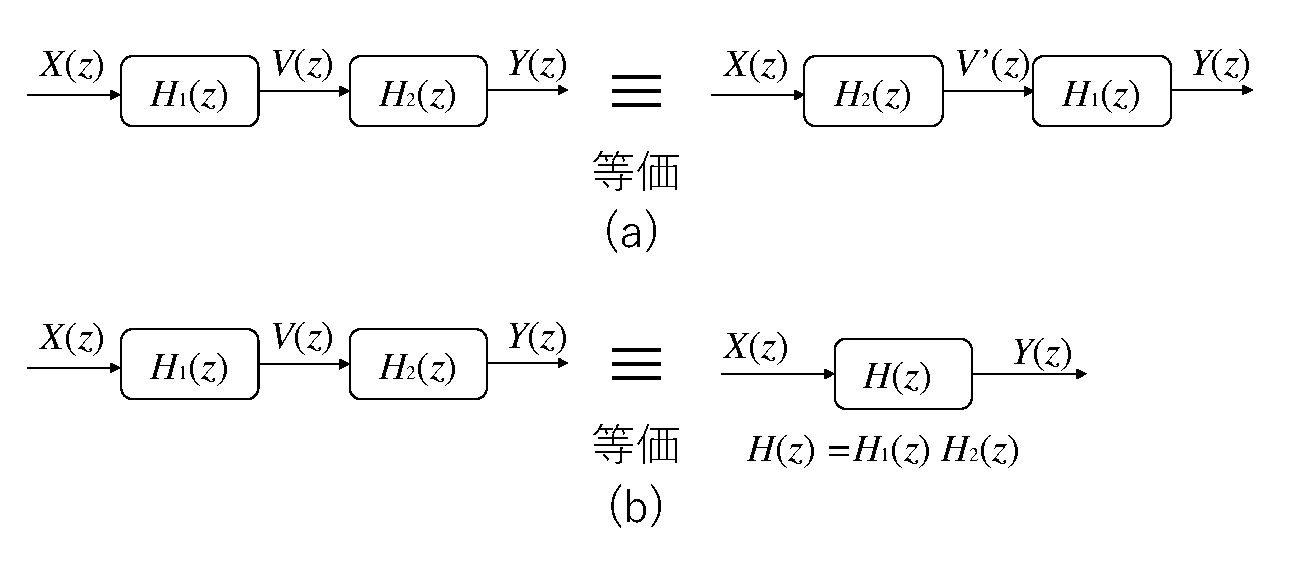
\includegraphics[width=10cm]{fig/zu-3-17.eps}
\end{center}
\caption{システムの縦続型構成}
\label{fig:zu-3-17}
\end{figure}

\subsection{並列型構成}

図\ref{fig:zu-3-18}のように2つのシステムを構成することを,\index{へいれつがたこうせい@並列型構成}並列型構成という.この処理全体をひとつの伝達関数$H(z)$で表すと,
\begin{equation}
H(z)=H_1(z)+H_2(z)
\end{equation}
と書くことができる.たとえば,3点平均である式(\ref{eqn:eqn-3-61})の場合であれば,

\begin{eqnarray}
H(z)&=&H_1(z)+H_2(z) \nonumber \\
 &=&\frac{1}{3}(1+z^{-1}+z^{-2})+\frac{1}{3}(1+z^{-1}+z^{-2}) \nonumber \\
 &=&\frac{2}{3}(1+z^{-1}+z^{-2})
\end{eqnarray}\vskip.3\baselineskip

\noindent となる.

\begin{figure}[H]
\begin{center}
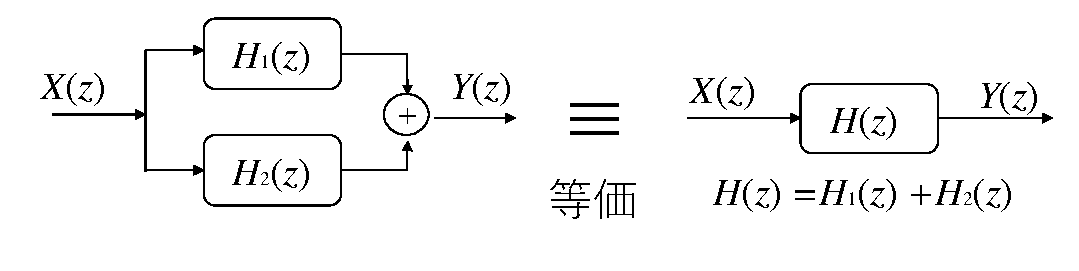
\includegraphics[width=10cm]{fig/zu-3-18.eps}
\end{center}
\caption{システムの並列型構成}
\label{fig:zu-3-18}
\end{figure}

\section*{演習問題}

\subsection*{問題\ref{chapter:42}.1}

以下の逆z変換を,べき級数展開法と部分分数展開法を用いて求めよ.

(1) $X(z)=z^2+2+2z^{-3}$

(2) $X(z)=\displaystyle \frac{1}{1-0.5z^{-1}}$

(3) $X(z)=\displaystyle \frac{2z^{-1}}{1-0.5z^{-1}} + \frac{1}{1-z^{-1}}$

(4) $X(z)=\displaystyle \frac{1}{(1-0.5z^{-1})(1-z^{-1})}$

\subsection*{問題\ref{chapter:42}.2}

以下のシステムの伝達関数を求め,ハードウェア構成を示せ.

(1) $y(n)=x(n)+ax(n-1)+bx(n-2)$

(2) $y(n)=x(n)+ax(n-1)+by(n-2)$

(3) $y(n)=x(n)+ay(n-1)+by(n-2)$

\subsection*{問題\ref{chapter:42}.3}

以下のシステムにおける周波数特性,伝達関数の極をそれぞれ求め,安定性を判別せよ.

(1) $H(z)=1+2z^{-1}+z^{-2}$

(2) $H(z)=\displaystyle \frac{1+2z^{-1}}{2+z^{-1}}$


